\chapter{Aufgabe 10}
\section{Aufgabe 10.1}

\paragraph{Aufgabenstellung}
Nutzen Sie das Beispiel aus Listing 1 bzw. die Beispiele aus dem B15-Git, um ein Programm zu schreiben welches zwei Betriebsmodi besitzt. In Zustand A sollen die digitalen Eingänge invertiert auf die digitalen Ausgänge weitergereicht werden. In Zustand B soll auf den digitalen Ausgängen das Lichtmuster aus dem Film Knightrider dargestellt werden. Unterscheiden Sie beide Betriebsmodi, indem Sie einen der DIP-Schalter auswerten.

\begin{wrapfigure}[20]{r}{.3\textwidth}
	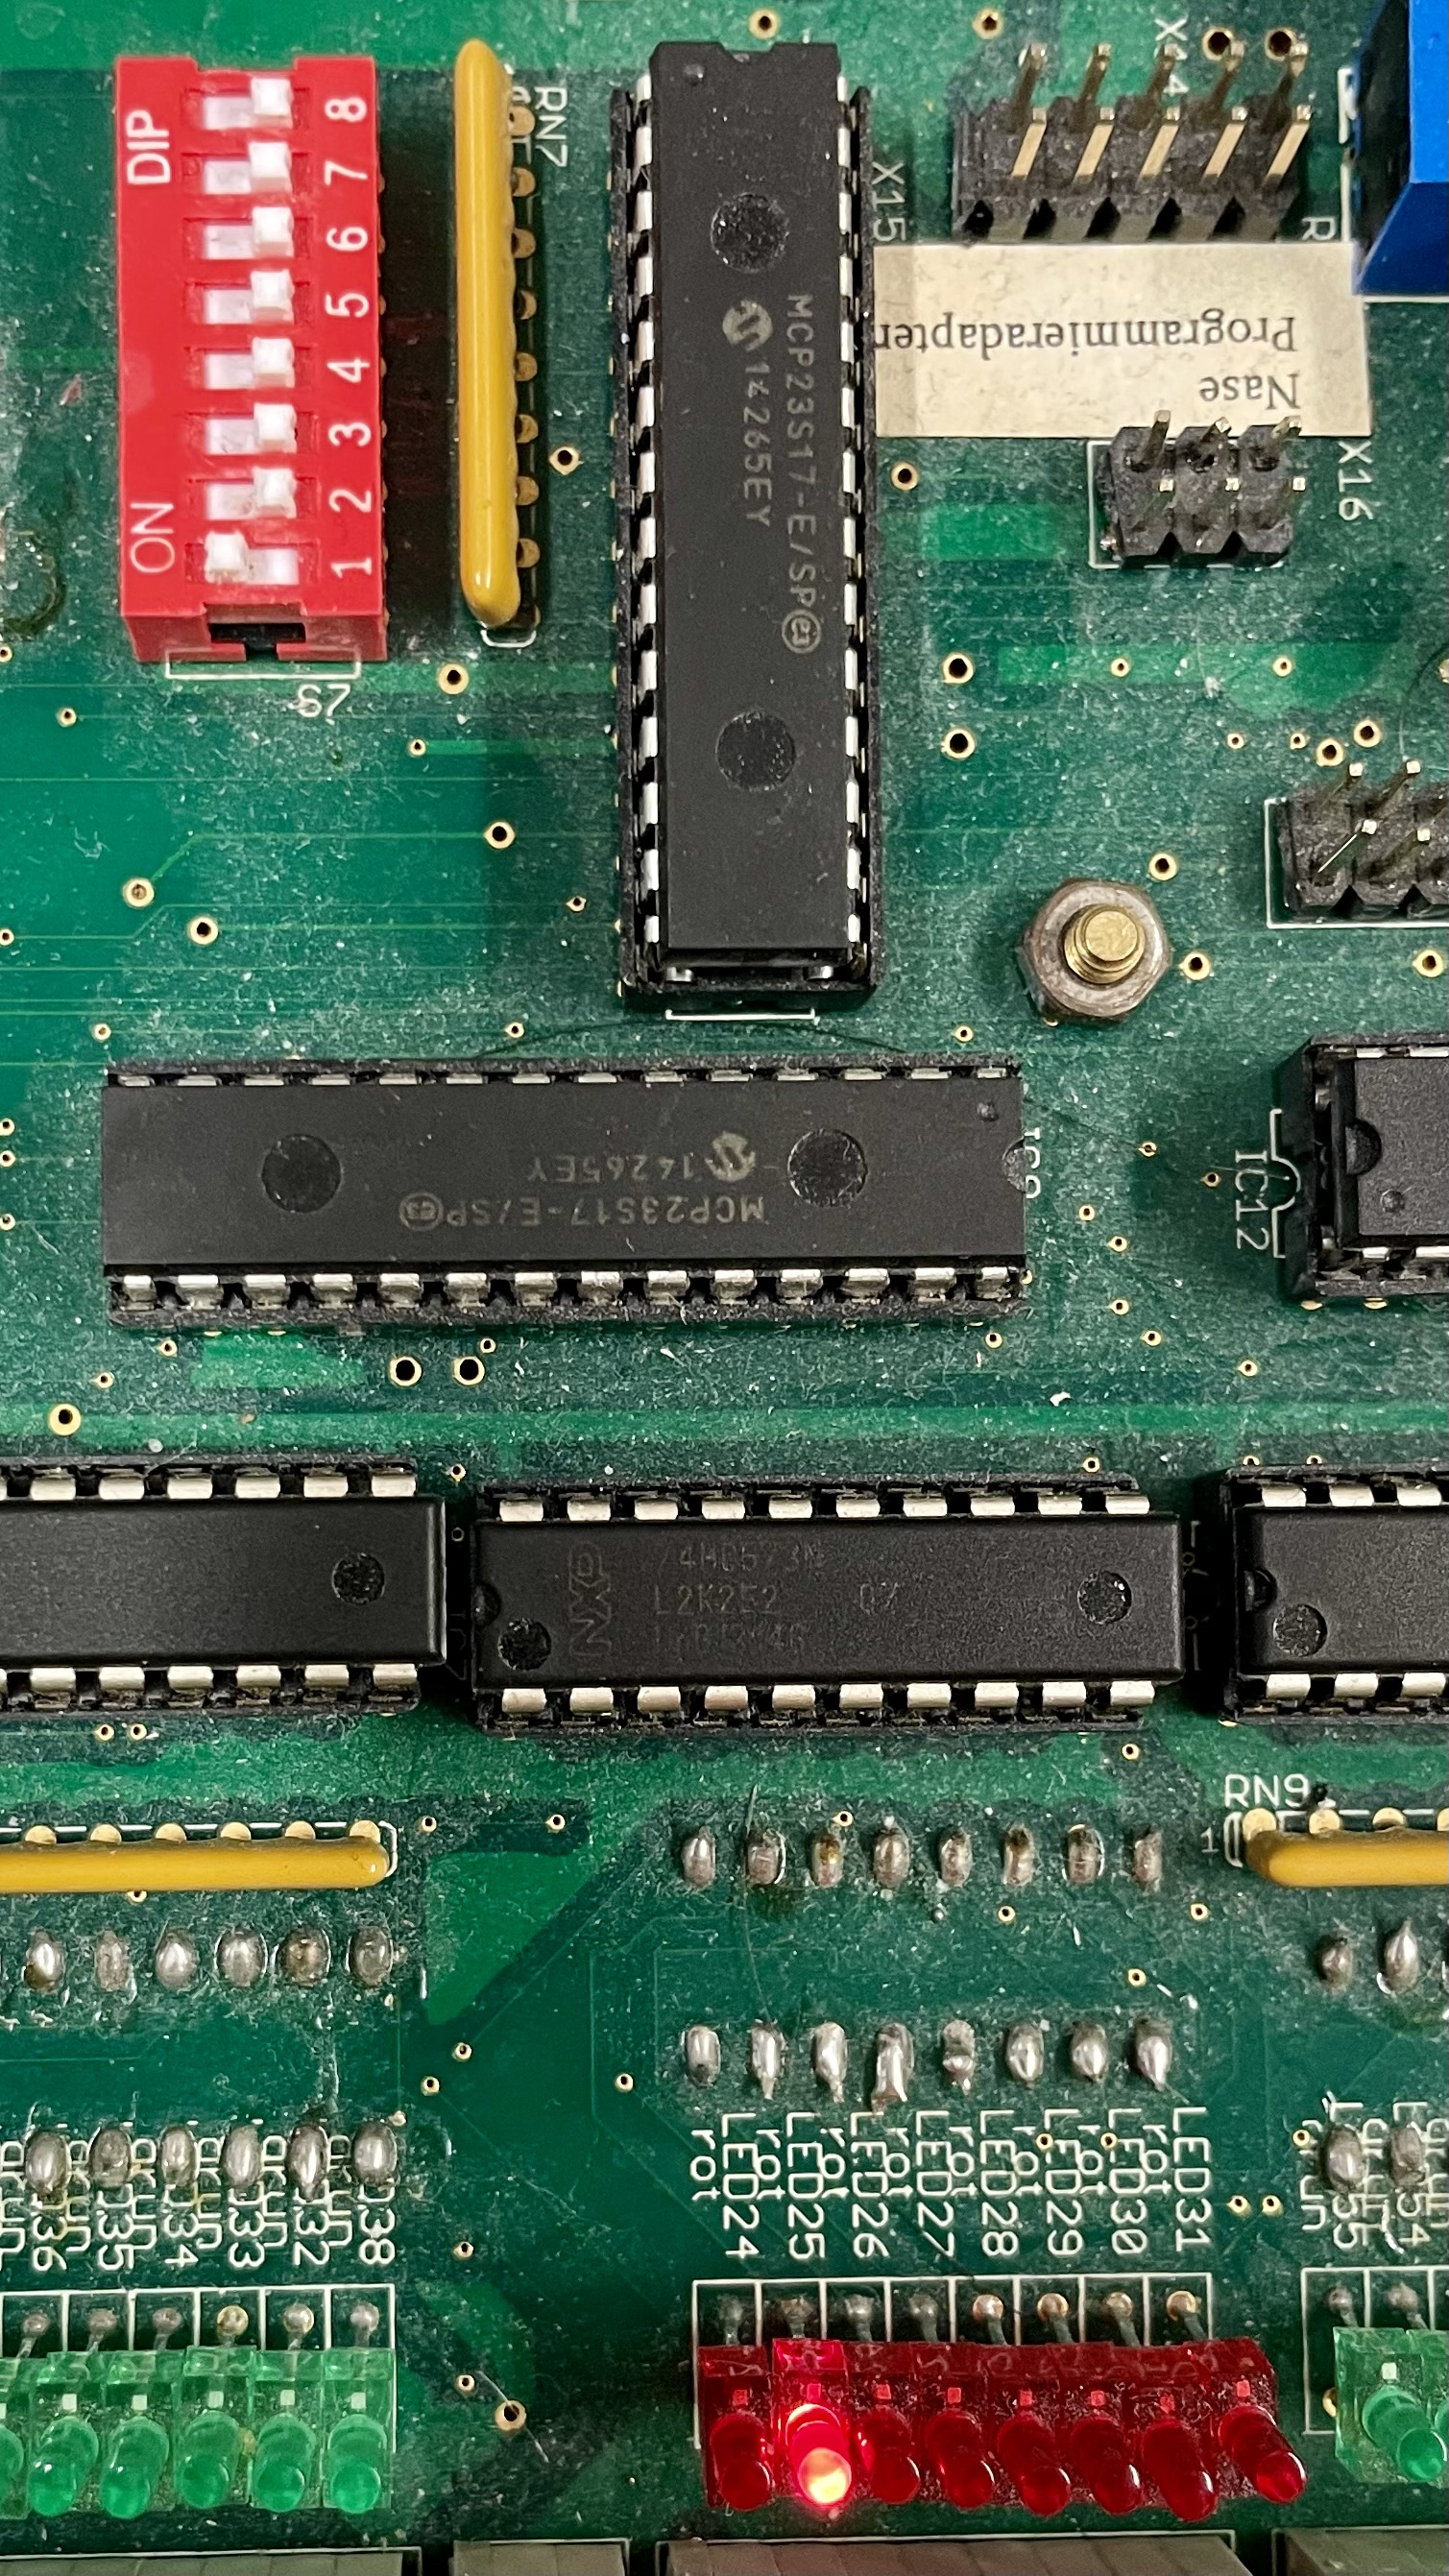
\includegraphics[width=.3\textwidth]{task10-1-B-switch.JPG}
	\caption{DIP-Schalter}
	\label{task10-1-B}
\end{wrapfigure}

\paragraph{Vorüberlegung}
Das B15-Board verfügt an allen BA und BE Steckleisten über 8 Anschlüsse. LEDs hinter den Anschlussbuchsen stellen die aktuelle Dezimalzahl in Binär da. Rechnet man $2^8$ ergibt dies 256, folglich können hier Zahlen von Null bis 255 Ein- sowie Ausgegeben werden. Um das Eingangssignal zu Invertieren, kann man daher einfach den Eingang von 255 subtrahieren. Das darzustellende Muster aus dem angegebenen Film ist ein einfaches hin- und herwandern einer einzelnen aktiven LED.

\paragraph{Durchführung}
In einer endlos laufenden Schleife soll der Wert des DIP-Schalters (in Abbildung \vref{task10-1-B} oben links), welcher Teil des B15-Boards ist, abgefragt und die entsprechenden Zustände ausgeführt werden. Steht der Schalter auf $0$, soll das Programm \textit{Zustand A} einmal ausführen. Sollte der Wert $1$ sein, wird \textit{Zustand B} einmal durchlaufen. In Zustand A wird der Wert des Blocks BE-0 ausgelesen, von 255 subtrahiert und das Ergebnis auf BA-0 geschrieben, wie in Abbildung \vref{task10-1-A} gezeigt. In Zustand B werden zwei Zählerschleifen nacheinander ausgeführt, welche den Dezimalwert der aktuellen LED halbieren bzw. verdoppeln und ihn mit einer leichten Verzögerung, die dem Knightrider Muster ähnelt, auf den Ausgang BA-0 schreibt. Der Quelltext kann nachfolgend entnommen werden.

\begin{figure}
	\begin{minipage}[c]{0.48\linewidth}
		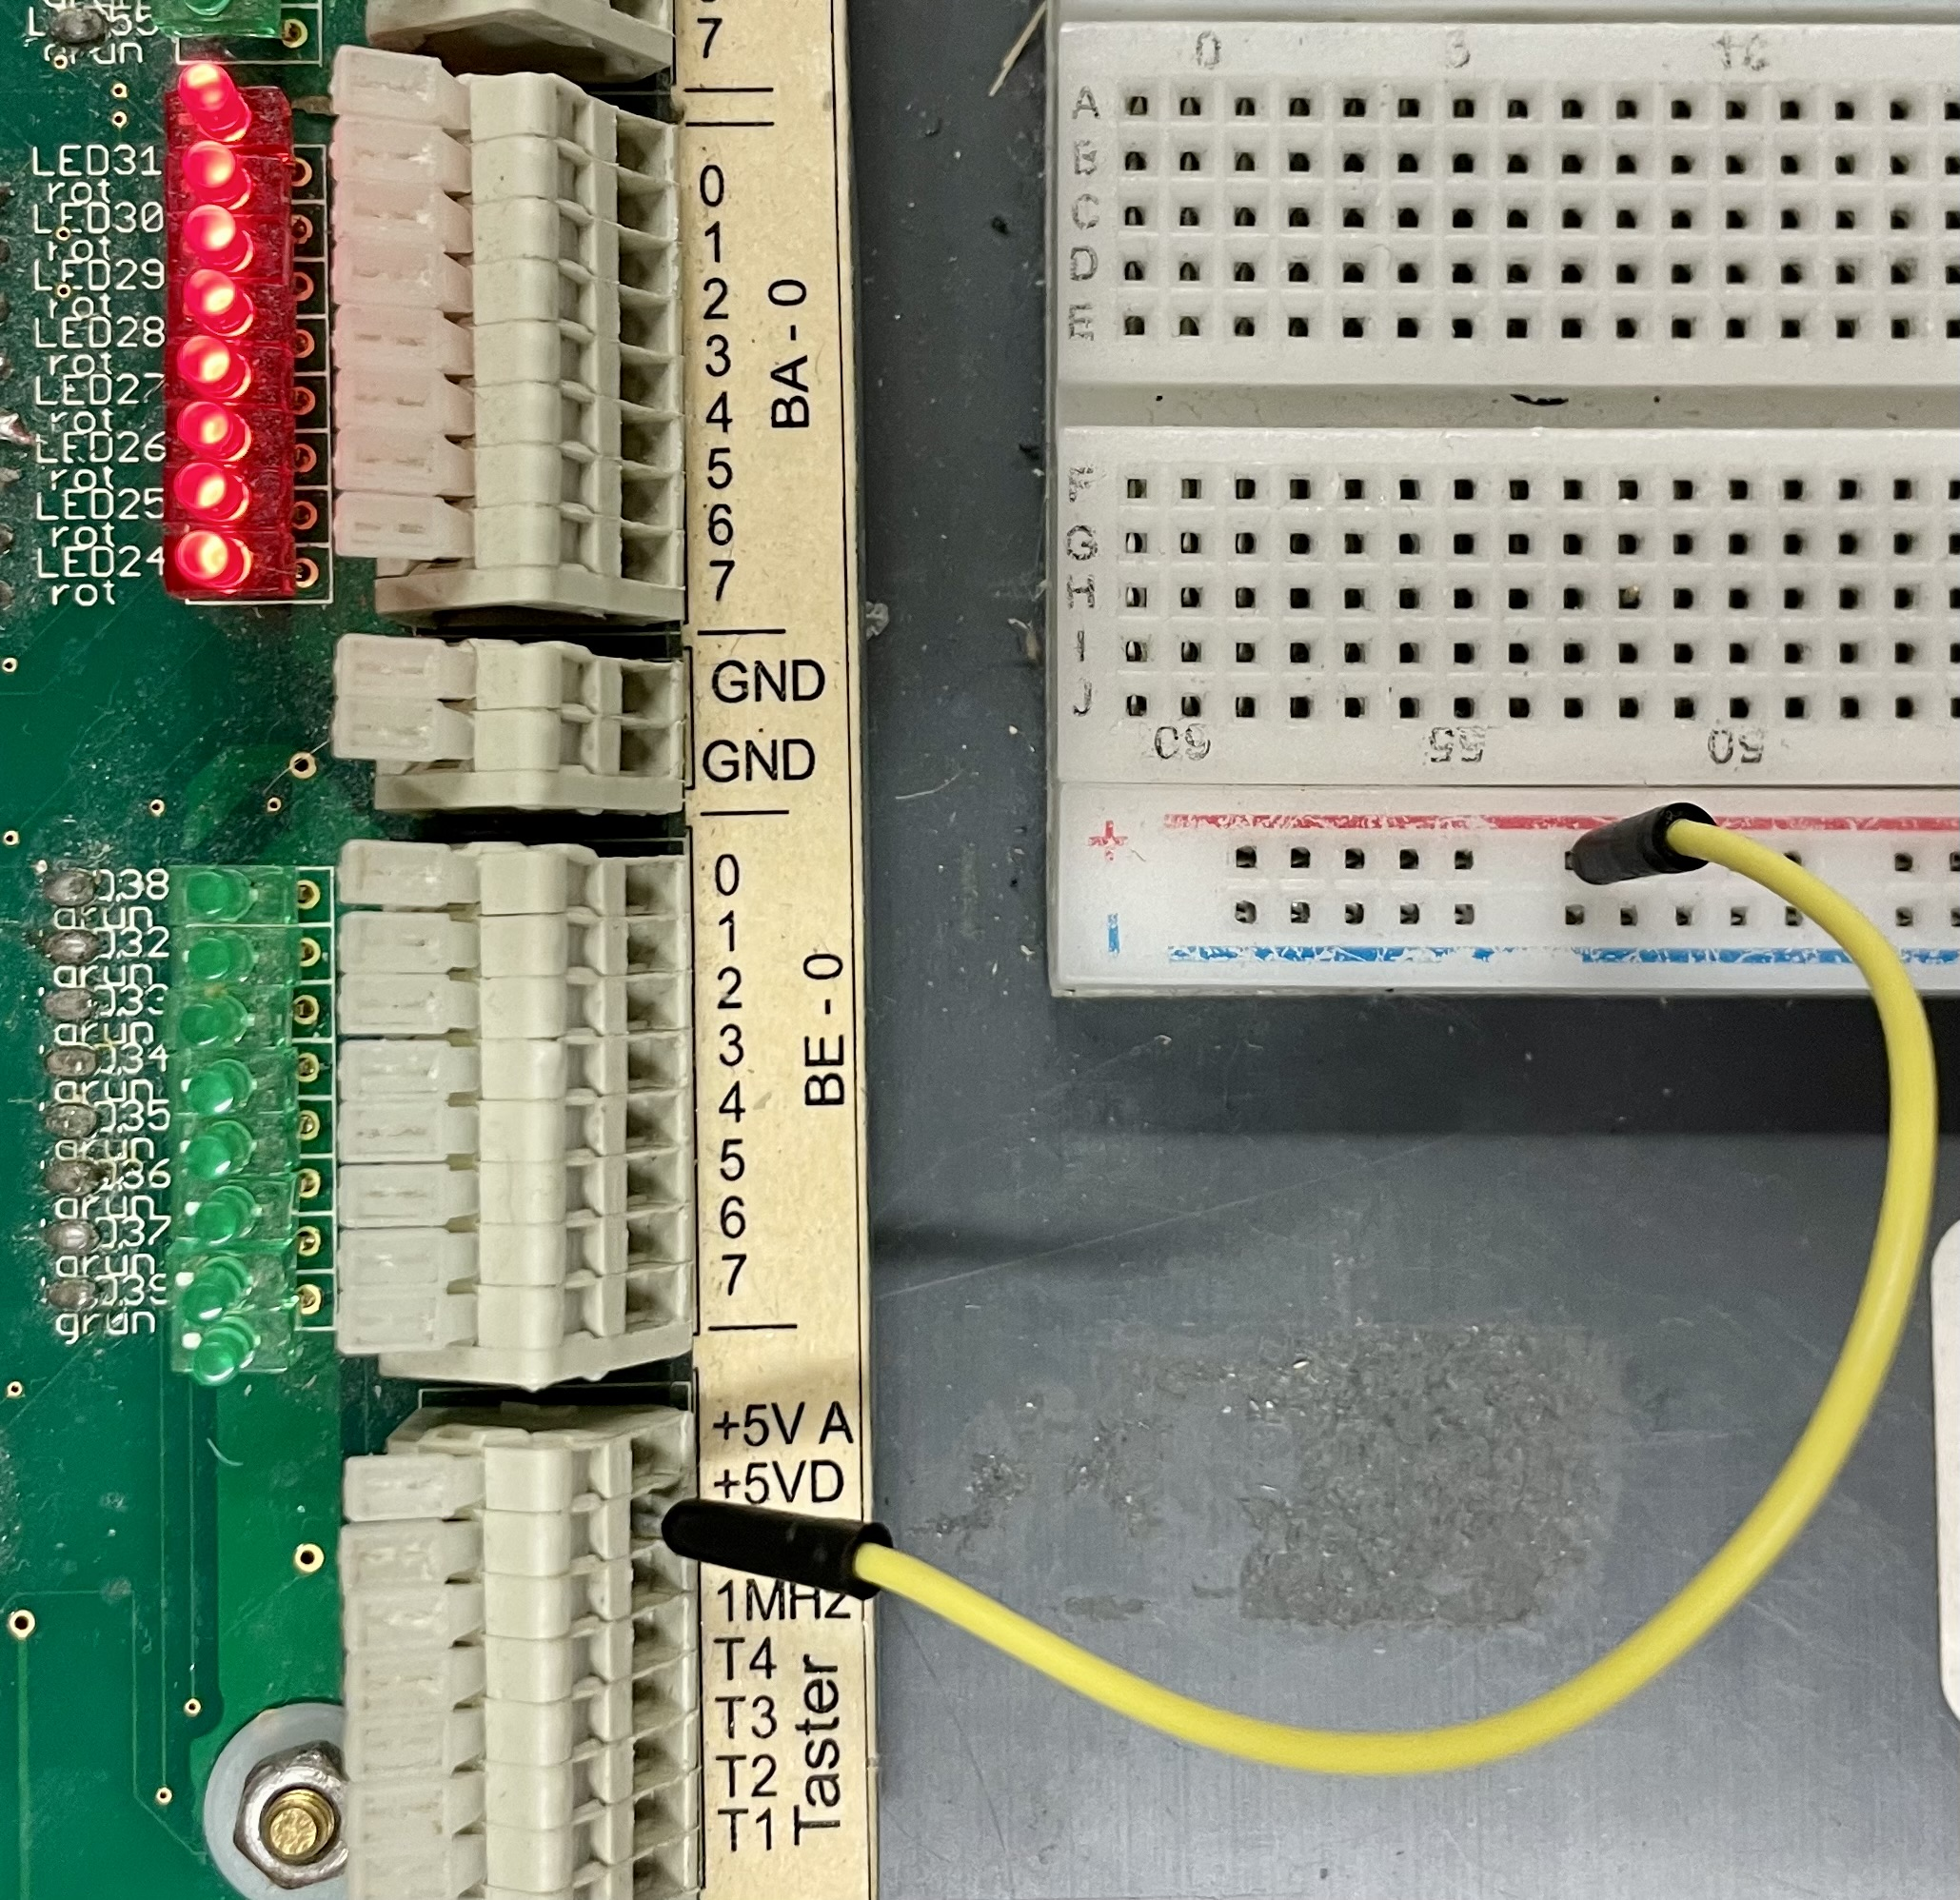
\includegraphics[width=\linewidth]{task10-1-A-0.JPG}
	\end{minipage}
	\hfill
	\begin{minipage}[c]{0.485\linewidth}
		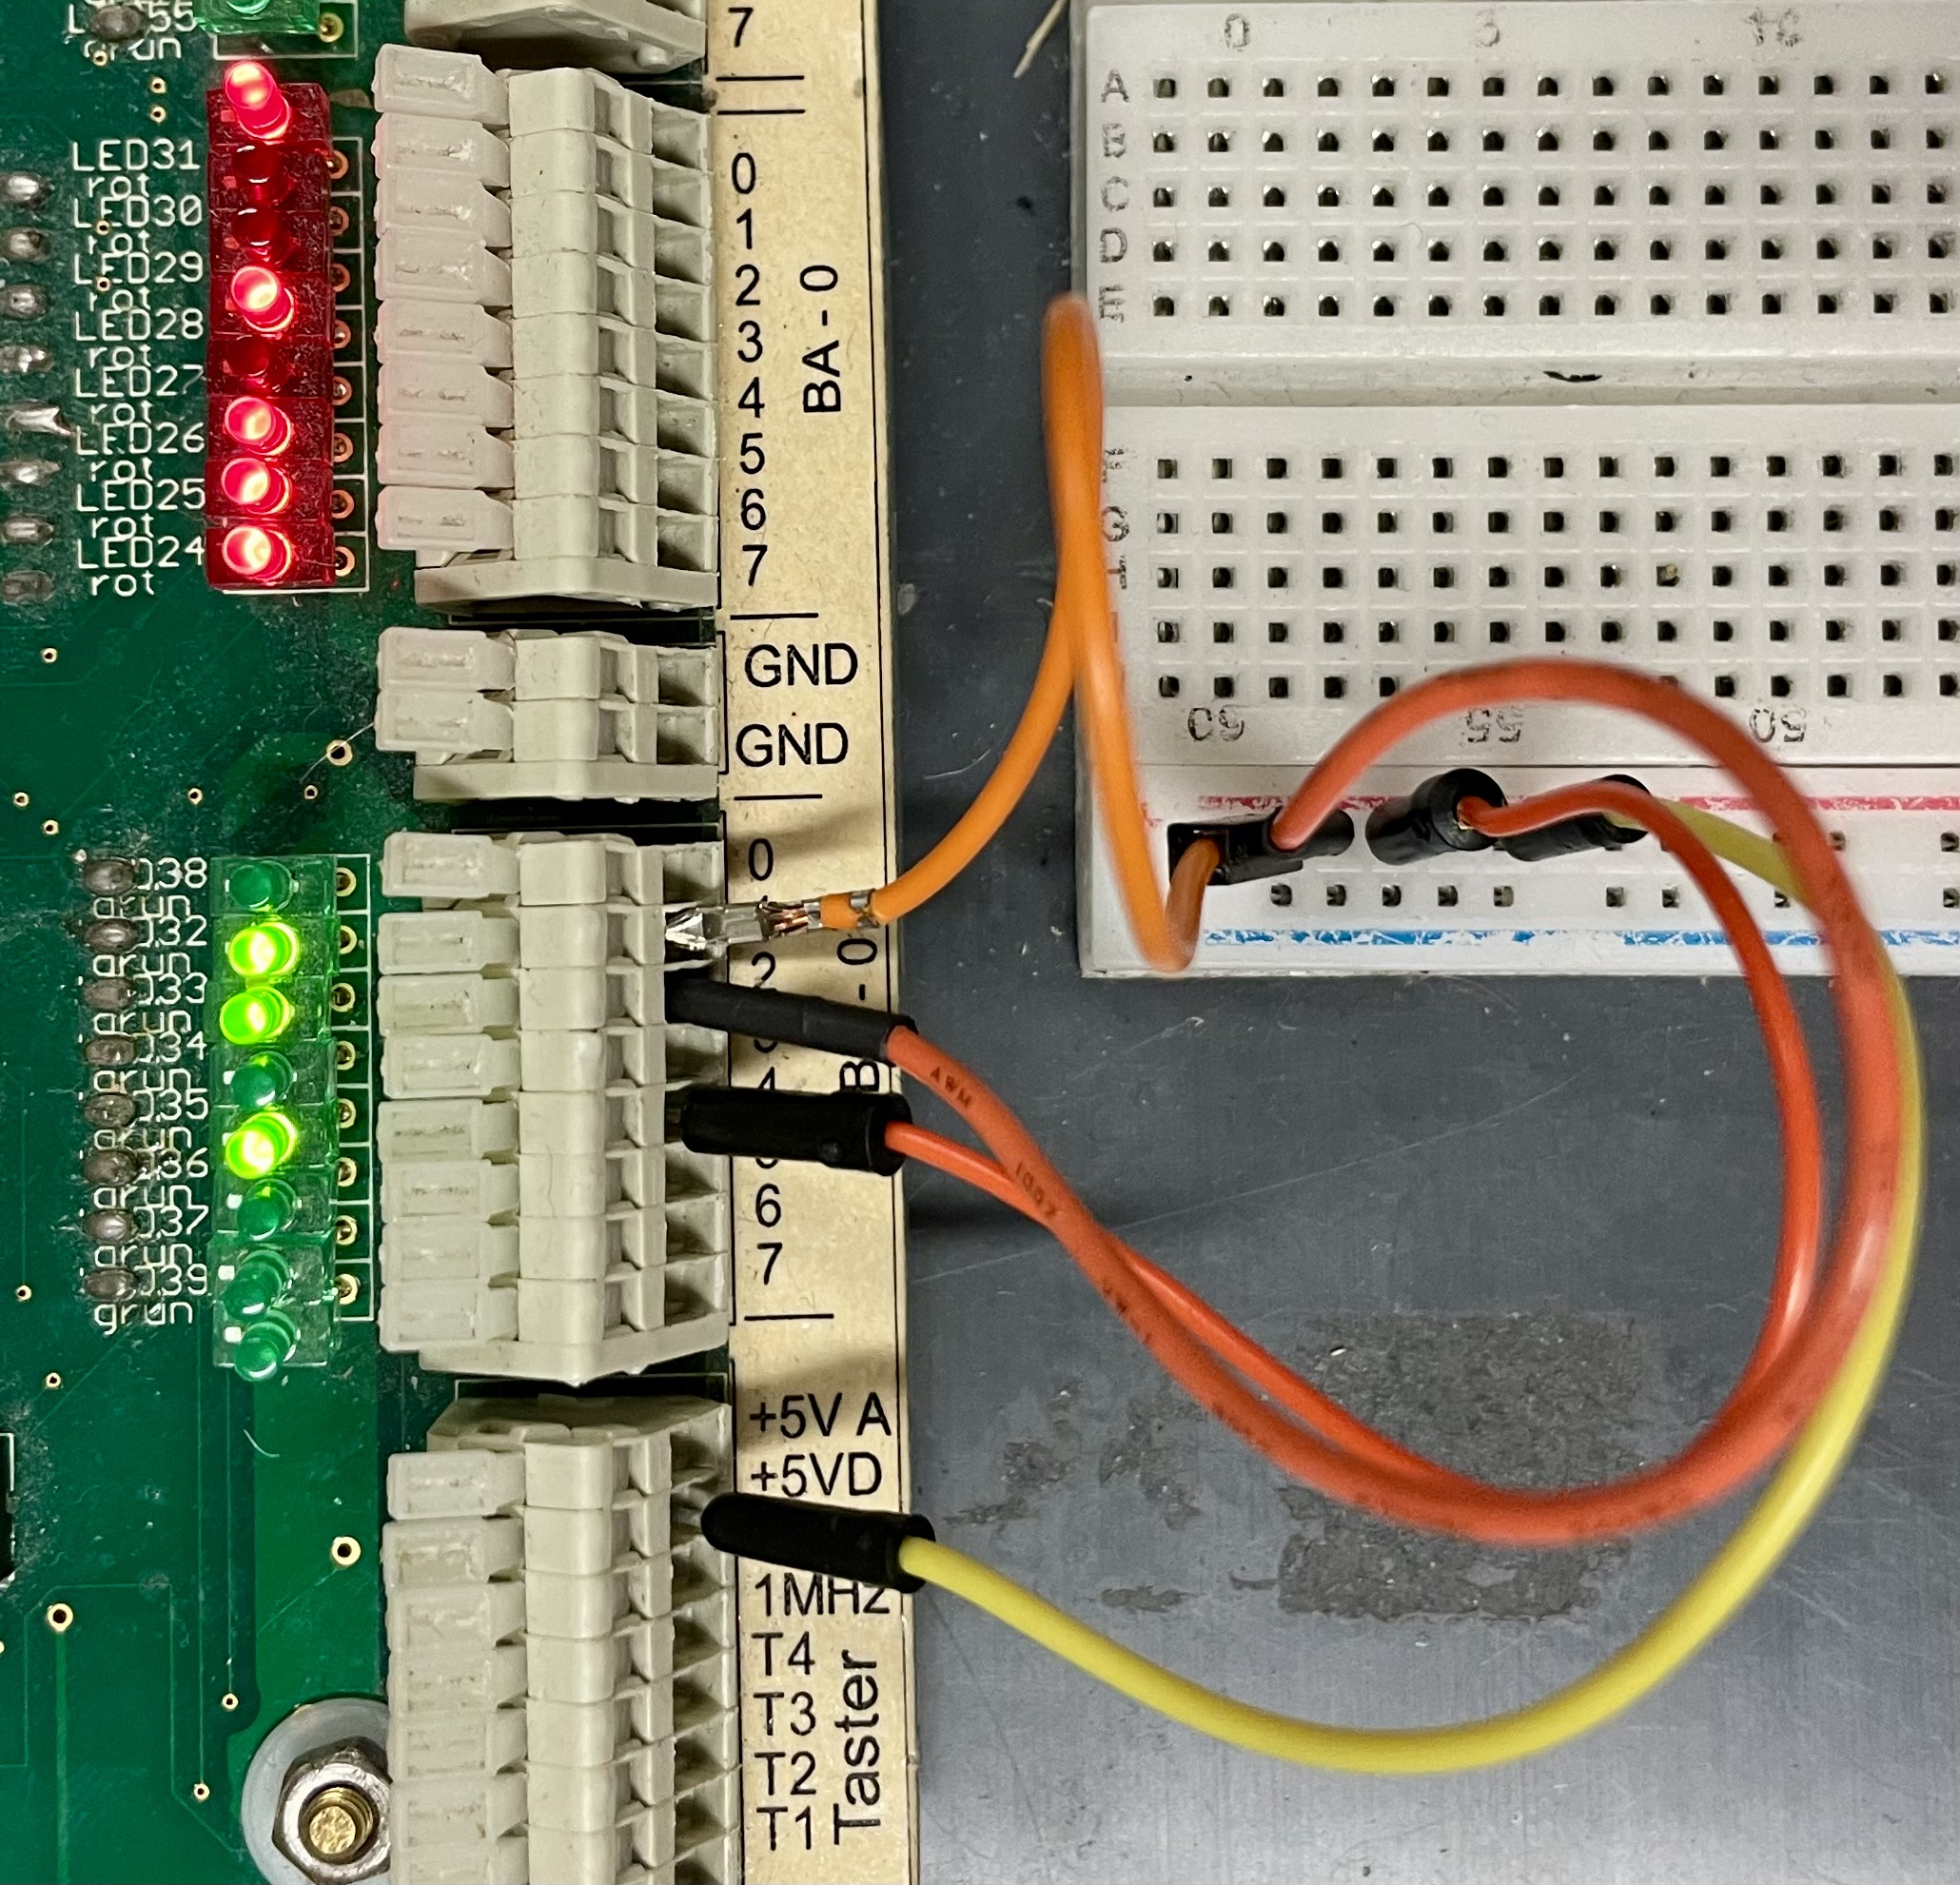
\includegraphics[width=\linewidth]{task10-1-A-1.JPG}
	\end{minipage}
	\caption{Zustand A}
	\label{task10-1-A}
\end{figure}

\def\ledspacing{0.13\linewidth}
\def\ledpath{/KnightRider_erleuchtete-LEDs/LED-}

\begin{figure}
	\begin{minipage}[c]{\ledspacing}
		\includegraphics[width=\linewidth]{\ledpath 0.png}
	\end{minipage}
	\hfill
	\begin{minipage}[c]{\ledspacing}
		\includegraphics[width=\linewidth]{\ledpath 1.png}
	\end{minipage}
	\hfill
	\begin{minipage}[c]{\ledspacing}
		\includegraphics[width=\linewidth]{\ledpath 2.png}
	\end{minipage}
	\hfill
	\begin{minipage}[c]{\ledspacing}
		\includegraphics[width=\linewidth]{\ledpath 3.png}
	\end{minipage}
	\hfill
	\begin{minipage}[c]{\ledspacing}
		\includegraphics[width=\linewidth]{\ledpath 4.png}
	\end{minipage}
	\hfill
	\begin{minipage}[c]{\ledspacing}
		\includegraphics[width=\linewidth]{\ledpath 5.png}
	\end{minipage}
	\hfill
	\begin{minipage}[c]{\ledspacing}
		\includegraphics[width=\linewidth]{\ledpath 6.png}
	\end{minipage}
	\\ \\
	\begin{minipage}[c]{\ledspacing}
	\includegraphics[width=\linewidth]{\ledpath 7.png}
	\end{minipage}
	\hfill
	\begin{minipage}[c]{\ledspacing}
	\includegraphics[width=\linewidth]{\ledpath 6.png}
	\end{minipage}
	\hfill
	\begin{minipage}[c]{\ledspacing}
	\includegraphics[width=\linewidth]{\ledpath 5.png}
	\end{minipage}
	\hfill
	\begin{minipage}[c]{\ledspacing}
	\includegraphics[width=\linewidth]{\ledpath 4.png}
	\end{minipage}
	\hfill
	\begin{minipage}[c]{\ledspacing}
	\includegraphics[width=\linewidth]{\ledpath 3.png}
	\end{minipage}
	\hfill
	\begin{minipage}[c]{\ledspacing}
	\includegraphics[width=\linewidth]{\ledpath 2.png}
	\end{minipage}
	\hfill
	\begin{minipage}[c]{\ledspacing}
	\includegraphics[width=\linewidth]{\ledpath 1.png}
	\end{minipage}
	
	\caption{Zustand B}
\end{figure}

\paragraph{Schlussfolgerung}
Das B15-Board verhält sich wie in der Aufgabenstellung gefordert und reagiert schnell. Sollte jedoch ein Wert größer als $1$ am DIP-Schalter eingestellt sein, wird nichts ausgeführt. Der Versuch ist erfolgreich.
\\\\
\inputminted[linenos=true, breaklines, fontsize=\fontsize{10pt}{10pt}]{cpp}{../task10/main.cpp}